\section{Related Work}\label{sec:related}

\textbf{Social-cognition and psychometric evaluation.} ToMBench~\citep{ToMBench}, FANToM~\citep{Kim2023_FANTOM}, OpenToM~\citep{Xu2024_OpenToM}, CogMir~\citep{CogMir}, CogBench~\citep{CogBench}, and PsychoBench~\citep{PsychoBench} score frozen models on curated items. Psychometric frameworks measure and shape LLM personality~\citep{SerapioGarcia2025_PsychometricLLM,Ye2025_LLM_Psychometrics}, expressed values shift with context~\citep{Kovac2024_StickToRole}, and the reliability of self-report inventories for LLMs is contested~\citep{Binz2023,Shu2024_PsychReliability,Gupta2024_SelfAssessment,Huang2024_ScaleReliability,Lee2025_TRAIT,Jiang2024_PersonaLLM,Han2025_PersonalityIllusion}. These works measure a snapshot and cannot separate what is in the weights from what an interaction history adds. SocCogEval places BFI-10~\citep{Rammstedt2007_BFI10,PsychoBench} and Asch-style items~\citep{Asch1956_Conformity} in a paired pre-post design, so scores become difference-in-differences statistics that read as transfer.

\textbf{Agent societies and multi-agent systems.} OASIS~\citep{OASIS}, AgentSociety~\citep{AgentSociety}, generative-agent worlds~\citep{Generative_Agents,Park2024_1000}, Concordia~\citep{Concordia}, SocioVerse~\citep{Li2024_SocioVerse}, and WarAgent~\citep{Hua2024_WarAgent} simulate LLM populations in which opinions~\citep{Chuang2024_OpinionDynamics,CisnerosVelarde2025_Funding}, cooperation~\citep{Piatti2024_GovSim}, conventions~\citep{FlintAshery2025_Conventions}, and individual personalities~\citep{Takata2024} emerge. SOTOPIA scores social skill within an episode~\citep{Zhou2024_SOTOPIA}, and LLM simulation is proposed as a social-science method~\citep{Anthis2025_SocialSim,Mou2024_SocialSimSurvey}. Debate, evaluation, and collaboration frameworks build teams from one model~\citep{Du2024_MultiagentDebate,Liang2024_DivergentDebate,Du2024_Debate,Smit2024_MAD,Chan2024_ChatEval,Li2023_CAMEL,Wu2024_AutoGen,Hong2024_MetaGPT}, often with persistent memory~\citep{MemGPT,Xu2025_AMEM,Mem0}. These studies inject heterogeneous priors or report collective outcomes, so they cannot isolate what interaction does to each agent. Controlled clones and a factorial contrast schema remove that confound.

\textbf{Drift, stability, and conformity.} Instructions fade within a dialog~\citep{Li2024_PersonaDrift}, reliability drops over multi-turn conversations~\citep{Laban2025_LostMultiTurn}, models agree with interlocutors~\citep{Sharma2024_Sycophancy} and conform to majorities~\citep{Weng2025_Conformity}, multi-agent systems fail through coordination errors~\citep{Cemri2025_MASFailures}, and a peer's presence changes behavior~\citep{Potter2026}. Rath~\citep{Rath2026_AgentDrift} defines drift as progressive degradation of task quality, coordination, and inter-agent coherence through a twelve-component Agent Stability Index. These works measure instability on the task or in the dialog (human parallels in Appendix~\ref{app:related}). We instead test distributional exchangeability of bit-identical clones. Initialization and brief assignment stay fixed, and we ask whether interaction transfers to off-topic response profiles under matched brief-only and no-interaction controls.

\textbf{Uncertainty in evaluation.} Observations within one unit are not independent replicates~\citep{Hurlbert1984}, items that share a source need clustered errors~\citep{Miller2024_ErrorBars,Cameron2015}, and synthetic samples can understate variation~\citep{Bisbee2024}. Multi-turn agent evaluation has mostly targeted task success~\citep{Yao2023_ReAct,MT-bench,AgentBench}. We treat the run as the unit of replication.

\begin{figure}[t]
\centering
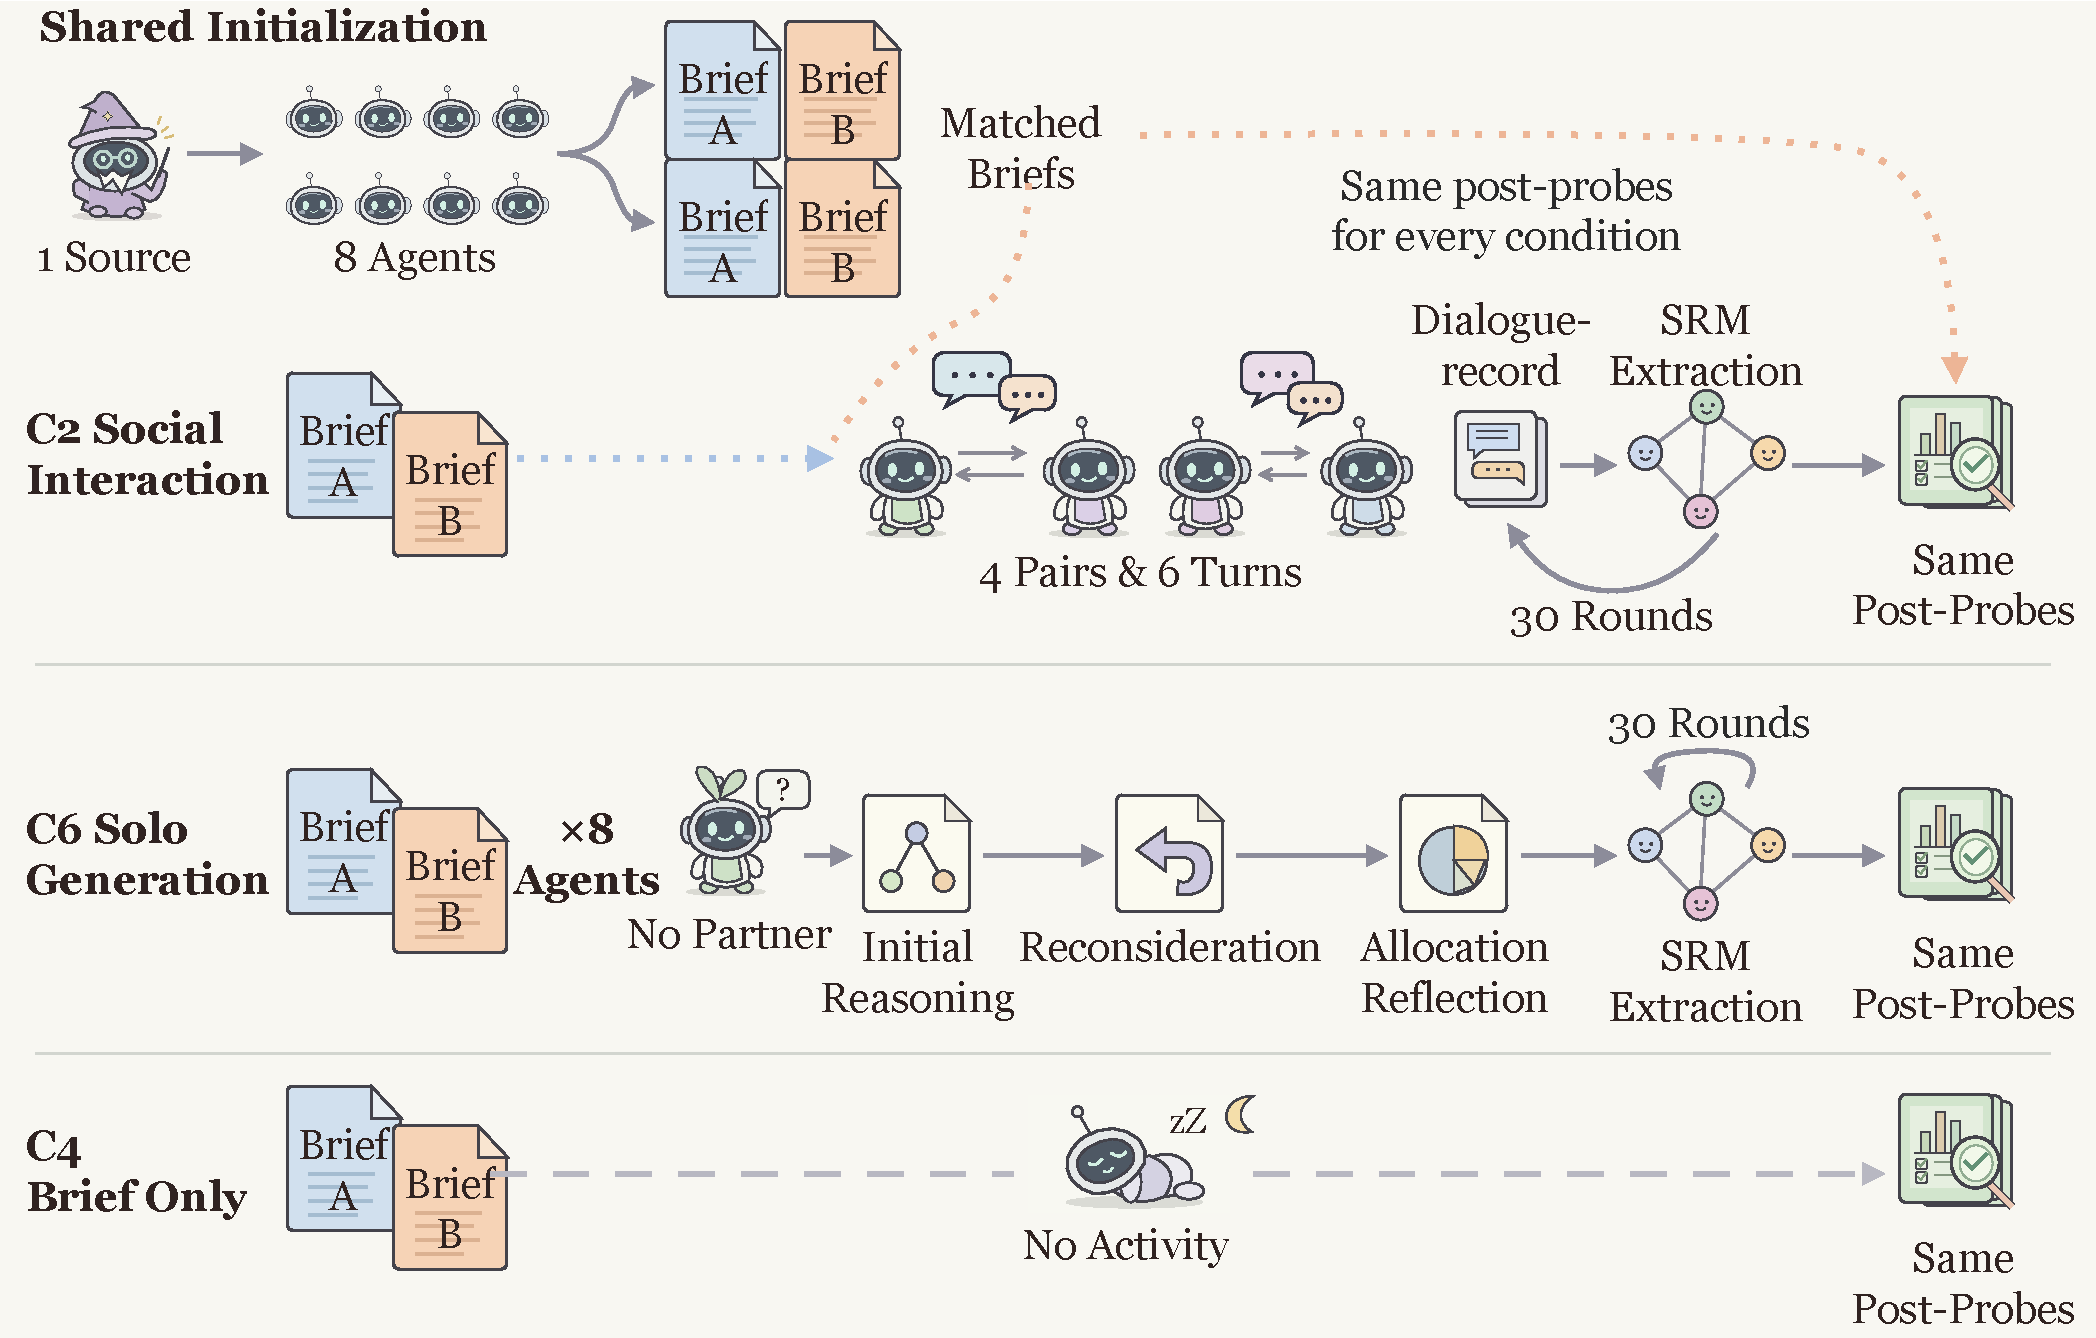
\includegraphics[width=\textwidth]{figures/fig4_c6.pdf}
\caption{The three comparison lanes. $C_6$ matches the $C_2$ call budget without a partner.}\label{F3sch}
\end{figure}
